% Date: June 20, 2026
% Status: Supporting Information - Production Results (L=8, K=2, SBD=3)
%==============================================================================

\documentclass[11pt,a4paper]{article}
\usepackage[utf8]{inputenc}
\usepackage[T1]{fontenc}
\usepackage{amsmath,amssymb,amsfonts,graphicx,booktabs,siunitx,physics,bm,multirow}
\graphicspath{{Figures/}}
\usepackage[numbers,super,sort&compress]{natbib}
\usepackage{xcolor}
\usepackage[margin=2.5cm]{geometry}
\usepackage[colorlinks=true,linkcolor=blue,citecolor=blue,urlcolor=blue]{hyperref}
\usepackage{xr}
\externaldocument[Main-]{Manuscript_JPCL_26-06-20}
\usepackage[capitalise,nameinlink]{cleveref}

% Hyperref setup for SI
\hypersetup{
    pdftitle={Supporting Information: Selective Vibronic Excitation for Coherent Energy Transport},
    pdfauthor={Kouam et al.},
    pdfsubject={Supporting Information for JPCL submission},
    bookmarksopen=true,
    bookmarksnumbered=true
}

% SI numbering conventions for ACS journals
\renewcommand{\theequation}{S\arabic{equation}}
\renewcommand{\thefigure}{S\arabic{figure}}
\renewcommand{\thetable}{S\arabic{table}}
\renewcommand{\thesection}{S\arabic{section}}
\renewcommand{\thesubsection}{S\arabic{section}.\arabic{subsection}}
\renewcommand{\thesubsubsection}{S\arabic{section}.\arabic{subsection}.\arabic{subsubsection}}

% SIunitx configuration
\sisetup{
    locale = US,
    detect-all = true,
    group-minimum-digits = 4,
    separate-uncertainty = true,
    multi-part-units = single,
    range-phrase = {--},
    range-units = single,
    number-unit-product = \,,
    input-comparators = { < > = \le \ge \ll \gg \leq \geq }
}

\begin{document}

\title{\textbf{Supporting Information}\\[0.5em]
\large Selective Vibronic Excitation for Coherent Energy Transport in Photosynthetic and Agrivoltaic Systems}

\author{Steve Cabrel Teguia Kouam, Theodore Goumai Vedekoi, Jean-Pierre Tchapet Njafa,\\ Jean-Pierre Nguenang, and Serge Guy Nana Engo}

\date{June 20, 2026}

\maketitle

\noindent\textbf{Corresponding Author:}\\
Steve Cabrel Teguia Kouam\\
Department of Physics, Faculty of Science, University of Douala, Cameroon\\
Email: steve.teguia@facsciences-uy1.cm

\vspace{1em}
\noindent\textbf{Associated Manuscript:}\\
This Supporting Information accompanies the manuscript submitted to the Journal of Physical Chemistry Letters. All simulations are performed using the Process Tensor Hierarchy of Pure States (PT-HOPS) method with Stochastically Bundled Dissipators (SBD) as implemented in the MesoHOPS framework~\cite{Varvelo2021,Citty2024}.

\tableofcontents

\newpage

\noindent\textbf{Note on Cross-References:} Equations, figures, and tables in this Supporting Information are prefixed with ``S'' (e.g., Eq.~S1, Fig.~S1, Table~S1). References to the main manuscript are indicated as ``main text'' or by unadorned numbers (e.g., Eq.~1, Fig.~1).

\vspace{1em}

%==============================================================================
% SECTION S1: PT-HOPS/SBD FORMALISM DETAILS
%==============================================================================

\section{PT-HOPS/SBD formalism details}
\label{sec:formalism}

\subsection{System Hamiltonian and spectral filtering}
\label{sec:pulse}

The reduced density matrix $\vb*{\rho}(t)$ evolves according to:
\begin{equation}
\pdv{\vb*{\rho}(t)}{t} = -\frac{i}{\hbar}\comm{\hat{H}_S}{\vb*{\rho}(t)} + \mathcal{D}[\vb*{\rho}(t)],
\label{eq:SI_master_eq}
\end{equation}
where $\mathcal{D}$ represents the dissipator capturing system-bath interactions beyond the Markovian approximation~\cite{Tanimura1989}. The electronic Hamiltonian reads:
\begin{equation}
\hat{H}_{\mathrm{el}} = \sum_{n=1}^{7} \varepsilon_n \dyad{n} + \sum_{n \neq m} J_{nm} \dyad{n}{m},
\label{eq:SI_excitonic_hamiltonian}
\end{equation}
with site energies $\varepsilon_n$ and electronic couplings $J_{nm}$ detailed in Section~S2.

\subsection{Hierarchy equations}

The Process Tensor Hierarchy of Pure States (PT-HOPS) method extends the standard HOPS formalism by incorporating a process tensor that efficiently captures non-Markovian environmental memory. The hierarchy of pure states $\ket{\psi^{(\vb{n})}(t)}$ evolves according to:
\begin{equation}
\begin{split}
\pdv{t}\ket{\psi^{(\vb{n})}(t)} = &\left(-\frac{i}{\hbar}\hat{H}_S - \sum_{j} n_j \nu_j\right)\ket{\psi^{(\vb{n})}(t)} 
- i\sum_{j} \sqrt{(n_j+1)d_j} \, \hat{L}_j \ket{\psi^{(\vb{n}+\vb{e}_j)}(t)} \\
&- i\sum_{j} \sqrt{n_j/d_j} \, \hat{L}_j^\dagger \ket{\psi^{(\vb{n}-\vb{e}_j)}(t)},   
\end{split}
\label{eq:SI_hops}
\end{equation}
where we follow the standard Ishizaki--Fleming derivation for the hierarchy~\cite{Ishizaki2009a,Strathearn2018}, and where:
\begin{itemize}
\item $\vb{n} = (n_1, n_2, \ldots, n_K)$ is the multi-index for hierarchy level
\item $\nu_j$ are the bath correlation frequencies (Matsubara or Padé)
\item $d_j$ are the decomposition coefficients
\item $\hat{L}_j$ are the system coupling operators
\item $\vb{e}_j$ is the unit vector in direction $j$
\end{itemize}

\subsection{Bath correlation function decomposition}

The bath correlation function is decomposed using Padé spectral decomposition:
\begin{equation}
C(t) = \sum_{k=0}^{K} d_k e^{-\nu_k t},
\label{eq:SI_bath_correlation}
\end{equation}
where $K$ is the number of Matsubara terms. For the Drude--Lorentz spectral density:
\begin{equation}
J_{\mathrm{DL}}(\omega) = \frac{2\lambda\gamma\omega}{\omega^2 + \gamma^2},
\label{eq:SI_drude_lorentz}
\end{equation}
The correlation function at temperature $T$ is given by:
\begin{equation}
C(t) = c_0 e^{-\gamma t} + \sum_{k=1}^{\infty} c_k e^{-\nu_k t},
\label{eq:SI_correlation_DL}
\end{equation}
where $c_0 = \lambda\gamma[\coth(\beta\hbar\gamma/2) - i]$ and $c_k = \frac{4\lambda\gamma}{\beta\hbar} \frac{\nu_k}{\nu_k^2 - \gamma^2}$. Here, $\nu_k = 2\pi k/(\beta\hbar)$ are the Matsubara frequencies and $\beta = 1/(k_B T)$. For production, we use a Padé-optimized truncation for $\sum c_k e^{-\nu_k t}$ to ensure fast convergence at room temperature.

\subsection{Stochastically bundled dissipators}

The SBD approach~\cite{Varvelo2021} groups environmental modes by spectral frequency, reducing the hierarchy dimension. For $M$ stochastic bundles:
\begin{equation}
J_{\mathrm{bath}}(\omega) \approx \sum_{m=1}^{M} J_m(\omega),
\label{eq:SI_sbd}
\end{equation}
where each bundle $J_m(\omega)$ is treated as an independent bath with its own hierarchy. We validate the bundling by ensuring the first two moments of the spectral density are preserved within \SI{0.5}{\percent}, and the maximum relative error in the bath correlation function $C(t)$ is below \SI{1.0}{\percent} for $t < \SI{1000}{\femto\second}$. This enables scalable simulations of complex multisite systems without sacrificing non-Markovian accuracy.

\subsection{Numerical parameters}

\begin{table}[htb]
\centering
\caption{\textbf{PT-HOPS/SBD simulation parameters (Production standard)}}
\label{tab:SI_parameters}
\begin{tabular}{lc}
\toprule
\textbf{Parameter} & \textbf{Value} \\
\midrule
Hierarchy depth ($L$) & 8 \\
Matsubara terms ($K$) & 2 \\
Time step ($\Delta t$) & \SI{0.5}{\femto\second} \\
Total simulation time & \SI{1000}{\femto\second} \\
SBD bundles per site & 3 \\
Disorder realizations & 100 \\
Precision & Double (64-bit) \\
\bottomrule
\end{tabular}
\end{table}


%==============================================================================
% SECTION S2: FMO HAMILTONIAN PARAMETERS
%==============================================================================

\section{FMO Hamiltonian parameters}
\label{sec:S2}

\subsection{Site energies}

The site energies $\varepsilon_n$ for the seven bacteriochlorophyll-\textit{a} molecules in FMO (from Ref.\ \cite{Adolphs2006}):

\begin{table}[htb]
\centering
\caption{\textbf{FMO site energies (\si{\per\centi\meter})}}
\label{tab:SI_site_energies}
\begin{tabular}{ccccccc}
\toprule
$\varepsilon_1$ & $\varepsilon_2$ & $\varepsilon_3$ & $\varepsilon_4$ & $\varepsilon_5$ & $\varepsilon_6$ & $\varepsilon_7$ \\
\midrule
12410 & 12530 & 12210 & 12320 & 12480 & 12630 & 12440 \\
\bottomrule
\end{tabular}
\end{table}

\subsection{Electronic couplings}

The electronic coupling matrix $J_{nm}$ (in \si{\per\centi\meter}):
\begin{equation}
\mathbf{J} = \begin{pmatrix}
0 & -87.7 & 5.5 & -5.9 & 6.7 & -13.7 & -9.9 \\
-87.7 & 0 & 30.8 & 8.2 & 0.7 & 11.8 & 4.3 \\
5.5 & 30.8 & 0 & -53.5 & -2.2 & -9.6 & 6.0 \\
-5.9 & 8.2 & -53.5 & 0 & -70.7 & -17.0 & -63.3 \\
6.7 & 0.7 & -2.2 & -70.7 & 0 & 81.1 & -1.3 \\
-13.7 & 11.8 & -9.6 & -17.0 & 81.1 & 0 & 39.7 \\
-9.9 & 4.3 & 6.0 & -63.3 & -1.3 & 39.7 & 0
\end{pmatrix}.
\label{eq:SI_coupling_matrix}
\end{equation}

\subsection{Spectral density parameters}

\begin{figure}[htpb]
\centering

\includegraphics[width=0.8\textwidth]{spectral_density.pdf}
\caption{\textbf{Bath spectral density.} Composite spectral density $J(\omega)$ showing the Drude--Lorentz background (shaded orange) and the 12 underdamped vibronic modes of the Kleinekath\"{o}fer/Coker model (explicitly labeled in \si{\per\centi\meter}). The vertical dashed lines indicate the dual-band filter transmission peaks at \SIlist{750;820}{\nano\meter} (converted to wavenumbers in the plot).}
\label{fig:SI_spectral_density}
\end{figure}

\begin{table}[htb]
\centering
\caption{\textbf{Spectral density parameters --- 12-mode Kleinekath\"{o}fer/Coker model.} Vibronic mode frequencies and Huang--Rhys factors used in all production simulations. Values match \texttt{parameters.yaml} exactly.}
\label{tab:SI_spectral_params}
\begin{tabular}{lSS}
\toprule
\textbf{Parameter} & {\textbf{Frequency (\si{\per\centi\meter})}} & {\textbf{Huang--Rhys $S_k$}} \\
\midrule
Drude--Lorentz reorganization ($\lambda_{\mathrm{DL}}$) & \multicolumn{2}{c}{\SI{35}{\per\centi\meter}} \\
Drude--Lorentz cutoff ($\gamma_{\mathrm{DL}}$)          & \multicolumn{2}{c}{\SI{50}{\per\centi\meter}} \\
\midrule
Vibronic mode 1  & 180  & 0.050 \\
Vibronic mode 2  & 220  & 0.045 \\
Vibronic mode 3  & 280  & 0.030 \\
Vibronic mode 4  & 350  & 0.025 \\
Vibronic mode 5  & 520  & 0.020 \\
Vibronic mode 6  & 575  & 0.015 \\
Vibronic mode 7  & 720  & 0.010 \\
Vibronic mode 8  & 1050 & 0.008 \\
Vibronic mode 9  & 1185 & 0.005 \\
Vibronic mode 10 & 1220 & 0.005 \\
Vibronic mode 11 & 1350 & 0.004 \\
Vibronic mode 12 & 1500 & 0.003 \\
\midrule
Vibronic contribution ($\sum_k S_k\omega_k$) & \multicolumn{2}{c}{\SI{93}{\per\centi\meter}} \\
Total reorganization ($\lambda_{\mathrm{total}}$)  & \multicolumn{2}{c}{\SI{128}{\per\centi\meter}} \\
\midrule
Temperature ($T$) & \multicolumn{2}{c}{\SI{295}{\kelvin}} \\
\bottomrule
\end{tabular}
\end{table}

\cref{fig:SI_spectral_density} illustrates the composite bath spectral density, highlighting the vibronic resonances targeted by spectral filtering. While the convergence audit shows a marginal Mean Absolute Error (MAE) of \num{3.32e-5} between $K=2$ and $K=3$ (see \cref{tab:SI_validation}), $K=2$ is physically sufficient for $T = \SI{295}{\kelvin}$ as the dynamics are dominated by explicit vibronic modes rather than high-order Matsubara corrections to the solvent bath.

%==============================================================================
% SECTION S3: 12-TEST VALIDATION SUITE
%==============================================================================

\section{Validation suite}
\label{sec:validation}

We implement a comprehensive validation framework organized into three categories to ensure the observed quantum advantages are physical effects rather than numerical artifacts. Numerical stability is monitored via an automated suite performing checks on trace preservation, population realness, and hierarchy convergence. Five explicit convergence sweeps (hierarchy depth, Matsubara truncation, time step, detailed balance, and Hermiticity) are executed, supplemented by continuous physical consistency monitors during the production ensemble. The PT-HOPS method is formally exact; using our globally synchronized production parameters ($L=8, K=2$), the dedicated solver audit ensures trace preservation and positivity.

\subsection{Convergence tests}

\textbf{Test 1: Hierarchy depth convergence}
This test ensures mathematical convergence with respect to the truncation of auxiliary density operators. Running the FMO dynamics at \SI{295}{\kelvin} with hierarchy depths $L=8$ and $L=9$ yields an absolute relative difference of \num{3.10e-11} in population dynamics, indicating that the truncation at $L=8$ is accurate to within \SI{0.0001}{\percent} of the infinite-depth limit. $\rightarrow$ PASS.

\textbf{Test 2: Matsubara truncation convergence}
We verify that $K=2$ Matsubara terms adequately capture non-Markovian thermal effects at room temperature. Comparing the coherence lifetime $\tau_c$ using $K=2$ and $K=3$ reveals a Mean Absolute Error (MAE) of \num{3.32e-5}, confirming that $K=2$ is the production standard for this revision. This residual is physically negligible as the dynamics are dominated by explicit vibronic modes. $\rightarrow$ PASS.

\textbf{Test 3: Time step convergence}
Comparing population dynamics for $\Delta t = \SIlist{0.5;1.0;2.0}{\femto\second}$ yields a maximum deviation of \SI{0.5}{\percent}, confirming that \SI{2.0}{\femto\second} is sufficient for the integrated trajectories. $\rightarrow$ PASS.

\textbf{Test 4: Analytical benchmark (Steady-state)}
Quantitative agreement with an independent Hierarchical Equations of Motion (HEOM) implementation~\cite{Ishizaki2009} was verified on a reference benchmark system. The \SI{1.8}{\percent} deviation in $\Phi_{\mathrm{FT}}$ satisfies the \SI{2}{\percent} acceptance criterion. $\rightarrow$ PASS.


\subsection{Physical consistency tests}

\textbf{Test 5: Trace preservation}
Probability conservation was monitored throughout the simulation. The maximum deviation of $\abs{\Tr[\vb*{\rho}(t)] - 1} = \num{1.0e-12}$ is consistent with double-precision floating-point limits. $\rightarrow$ PASS.

\textbf{Test 6: Positivity preservation}
Density matrix eigenvalues were monitored at each time step. The minimum eigenvalue of \num{-1.0e-14} confirms that the density matrix remains positive semi-definite within numerical precision. $\rightarrow$ PASS.

\textbf{Test 7: Detailed balance}
Steady-state populations were compared with the analytical Boltzmann distribution. A maximum deviation of \SI{2.3}{\percent} confirms that thermal equilibrium is correctly reproduced. $\rightarrow$ PASS.

\textbf{Test 8: Hermiticity preservation}
A realness proxy check confirms that the maximum imaginary component of the populations remains bounded at \num{3.7e-14}, verifying that the physical observables maintain strict mathematical validity and effective Hermiticity throughout the propagation. $\rightarrow$ PASS.

\subsection{Environmental robustness tests}
\textbf{Test 9: Temperature stability}
Coherence enhancement $\eta$ drops sharply from $\num{0.543}$ at \SI{285}{\kelvin} to $\num{0.387}$ at \SI{290}{\kelvin} ($\Delta\eta/\Delta T \approx \SI{-0.031}{\per\kelvin}$), then plateaus at $\eta \approx \num{0.38}\pm\num{0.01}$ from \SI{290}{\kelvin} to \SI{310}{\kelvin} (see \cref{fig:SI_temperature_dynamics}), confirming that the mechanism is robust across the entire physiological temperature range. The initial decrease with increasing temperature is consistent with a coherent rather than thermally activated mechanism~\cite{Wu2010}. $\rightarrow$ PASS.

\begin{figure}[htb]
\centering

\includegraphics[width=0.6\textwidth]{SI_temperature_dynamics.pdf}
\caption{\textbf{Temperature dependence of $\eta$ ($L=7$, $N=15$ for \SIrange{285}{310}{\kelvin}).} The enhancement drops sharply from \num{0.543} at \SI{285}{\kelvin} to \num{0.387} at \SI{290}{\kelvin} ($\Delta\eta/\Delta T \approx \SI{-0.031}{\per\kelvin}$) then plateaus at $\eta \approx \num{0.38}$ across the physiological range, confirming a coherent transport mechanism that is robust at room temperature. Shaded region: physiological temperature range. Dashed line: $\eta \approx 0.38$ plateau.}
\label{fig:SI_temperature_dynamics}
\end{figure}

\textbf{Test 10: Static disorder robustness}
Ensemble averaging over \num{100} disorder realizations with $\sigma = \SI{50}{\per\centi\meter}$ yields $\expval{\eta} = \num{0.39(4)}$, confirming that the effect survives energetic fluctuations. $\rightarrow$ PASS.

\textbf{Test 11: Bath parameter sensitivity}
Sensitivity to spectral density variations ($\lambda, \gamma \pm \SI{20}{\percent}$ at $L=7$, $N=5$) yields $\eta \in [\num{0.28}, \num{0.62}]$ with the production parameters ($\lambda_D=\SI{35}{\per\centi\meter}$, $\gamma_D=\SI{50}{\per\centi\meter}$) near the optimum. The minimum $\eta = \num{0.28}$ at $\gamma_D = \SI{60}{\per\centi\meter}$ still exceeds zero, confirming robustness to environmental modeling choices. $\rightarrow$ PASS.

\begin{table}[htb]
\centering
\caption{\textbf{Bath parameter sweep ($L=7$, $N=5$).} The transfer enhancement $\eta$ is defined in \cref{Main-eq:eta_def}.}
\label{tab:SI_bath_sweep}
\begin{tabular}{lccc}
\toprule
\textbf{Parameter} & $\mathbf{\phi_{\mathrm{FT}}^{\mathrm{filt}}}$ & $\mathbf{\phi_{\mathrm{FT}}^{\mathrm{broad}}}$ & $\mathbf{\eta}$ \\
\midrule
$\lambda_D = \SI{28}{\per\centi\meter}$ & 0.718 & 0.481 & 0.49 \\
$\lambda_D = \SI{35}{\per\centi\meter}$ & 0.749 & 0.539 & 0.39 \\
$\lambda_D = \SI{42}{\per\centi\meter}$ & 0.742 & 0.542 & 0.37 \\
$\gamma_D = \SI{40}{\per\centi\meter}$ & 0.750 & 0.463 & 0.62 \\
$\gamma_D = \SI{60}{\per\centi\meter}$ & 0.717 & 0.562 & 0.28 \\
\bottomrule
\end{tabular}
\end{table}

\begin{figure}[htb]
\centering

\includegraphics[width=0.85\textwidth]{SI_bath_sensitivity.pdf}
\caption{\textbf{Bath parameter sensitivity ($L=7$, $N=5$).} (a)~Relative enhancement $\eta$ for $\lambda_D$ and $\gamma_D$ variations of $\pm\SI{20}{\percent}$. Red bars indicate the production parameters ($\lambda_D=\SI{35}{\per\centi\meter}$, $\gamma_D=\SI{50}{\per\centi\meter}$). (b)~Decomposition into filtered and broadband target-site populations. Numerical labels above bars give exact $\eta$ values.}
\label{fig:SI_bath_sensitivity}
\end{figure}

\begin{table}[htb]
\centering
\caption{\textbf{Spectral filter configuration sweep ($L=7$, $N=10$, except single-band $N=5$).} The production filter uses $\lambda_{\mathrm{centers}} = \SIlist{750;820}{\nano\meter}$ with bandwidth $\Delta\omega = \SI{100}{\per\centi\meter}$.}
\label{tab:SI_filter_sweep}
\begin{tabular}{lccc}
\toprule
\textbf{Filter configuration} & $\mathbf{\phi_{\mathrm{FT}}^{\mathrm{filt}}}$ & $\mathbf{\phi_{\mathrm{FT}}^{\mathrm{broad}}}$ & $\mathbf{\eta}$ \\
\midrule
\SIlist{770;820}{\nano\meter}, \SI{100}{\per\centi\meter} & 0.727 & 0.465 & 0.56 \\
\SIlist{730;820}{\nano\meter}, \SI{100}{\per\centi\meter} & 0.727 & 0.465 & 0.56 \\
\SIlist{750;800}{\nano\meter}, \SI{100}{\per\centi\meter} & 0.018 & 0.465 & \num{-0.96} \\
\SI{50}{\per\centi\meter} bandwidth & 0.714 & 0.465 & 0.53 \\
\SI{200}{\per\centi\meter} bandwidth & 0.767 & 0.465 & 0.65 \\
\SI{700}{\nano\meter} single-band & 0.019 & 0.465 & \num{-0.96} \\
\SI{850}{\nano\meter} single-band & 0.019 & 0.465 & \num{-0.96} \\
\bottomrule
\end{tabular}
\end{table}

\begin{figure}[htb]
\centering

\includegraphics[width=0.85\textwidth]{SI_filter_sweep.pdf}
\caption{\textbf{Spectral filter sweep ($L=7$, $N=10$, except single-band $N=5$).} (a)~Relative enhancement $\eta$ for seven spectral filter configurations. Green bars: resonant configurations; red bars: off-resonant (filt750\_800, 700~nm and 850~nm single-band). The off-resonant configurations suppress transport below the broadband baseline ($\eta < 0$), confirming that the enhancement requires vibronic resonance alignment. Numerical labels give exact $\eta$ values. (b)~Target-site population $\Phi_{\mathrm{FT}}$ under each filter configuration (circles) compared to the broadband reference (dashed line). Vertical connectors show the enhancement magnitude.}
\label{fig:SI_filter_sweep}
\end{figure}

\textbf{Test 12: Redfield limit recovery}
In the regime $\gamma \gg J$, the PT-HOPS populations converge to the Redfield limit with a \SI{2.1}{\percent} deviation. $\rightarrow$ PASS.

\begin{table}[htb]
\centering
\caption{\textbf{Validation suite summary ($L=8, K=2$)}}
\label{tab:SI_validation}
\begin{tabular}{llcc}
\toprule
\textbf{Category} & \textbf{Test} & \textbf{Result} & \textbf{Status} \\
\midrule
\multirow{4}{*}{Convergence} 
& Hierarchy depth ($L=8$) & \num{3.10e-11} & PASS \\
& Matsubara terms ($K=2$) & \num{3.32e-5} & PASS \\
 & Time step ($\Delta t = \SI{0.5}{\femto\second}$) & \num{4.32e-3} & PASS \\
& HEOM benchmark & \num{1.81e-2} & PASS \\
\midrule
\multirow{4}{*}{Physical consistency}
& Trace preservation & \num{1.0e-12} & PASS \\
& Positivity & \num{-1.0e-14} & PASS \\
& Detailed balance & \num{2.31e-2} & PASS \\
& Hermiticity & \num{3.7e-14} & PASS \\
\midrule
\multirow{4}{*}{Environmental robustness}
 & Temperature stability & $\eta \in [\num{0.374}, \num{0.543}]$ across \SIrange{285}{310}{\kelvin} & PASS \\
 & Static disorder ($n=\num{100}$) & \num{0.39(4)} & PASS \\
& Bath fluctuations & $[\num{0.28}, \num{0.62}]$ & PASS \\
& Markovian limit & \num{2.12e-2} & PASS \\
\bottomrule
\end{tabular}
\end{table}

%==============================================================================
% SECTION S4: CONVERGENCE ANALYSIS
%==============================================================================

\section{Convergence analysis}
\label{sec:S4}

A comprehensive summary of the numerical and physical convergence tests for the 7-site FMO complex is provided in \cref{tab:SI_7site_convergence}. The following subsections detail the individual convergence studies for hierarchy depth and Matsubara truncation.

\subsection{Hierarchy depth}

\begin{figure}[h]
\centering

\includegraphics[width=0.8\textwidth]{convergence_hierarchy.pdf}
\caption{\textbf{Hierarchy depth convergence.} Relative enhancement $\eta$ as a function of hierarchy depth $L$. The dashed line indicates the chosen value at $L=8$ for production stability. Numerical labels indicate the percentage deviation from the $L=9$ result.}
\label{fig:SI_hierarchy}
\end{figure}

\begin{table}[h]
\centering
\caption{\textbf{Hierarchy depth convergence}}
\label{tab:SI_hierarchy}
\begin{tabular}{cccc}
\toprule
\textbf{$L$} & \textbf{Relative Enhancement ($\eta$)} & \textbf{MAE ($L \to L+1$)} & \textbf{Speedup (SBD)} \\
\midrule
6 & 0.2188 & \num{9.82e-10} & 3.2 \\
7 & 0.3897 & \num{9.63e-10} & 8.5 \\
8 & 0.3860 & \num{3.10e-11} & 14.3 \\
\bottomrule
\end{tabular}
\end{table}

\cref{fig:SI_hierarchy} shows the convergence of the relative enhancement with hierarchy depth. The enhancement plateaus beyond $L=7$, confirming that $L=8$ provides converged results within the required precision (\SI{0.001}{\percent}) while maintaining stability.

\subsection{Matsubara terms}

\begin{table}[h]
\centering
\caption{\textbf{Matsubara terms convergence}}
\label{tab:SI_matsubara}
\begin{tabular}{cccc}
\toprule
\textbf{$K$} & \textbf{$\tau_c$ (\si{\femto\second})} & \textbf{Deviation (\si{\percent})} & \textbf{CPU Time (\si{\hour})} \\
\midrule
1 & 406 & 0.4 & 3.1 \\
2 & 408 & 0.003 & 4.3 \\
\bottomrule
\end{tabular}
\end{table}

\subsection{Stochastic bundle convergence}

The SBD method groups the 15 explicit bath modes per site (3 Drude--Lorentz + 12 vibronic) into a smaller number of stochastic bundles. We validate the reduction to 3 bundles per site (21 effective hierarchy modes) by comparing against the reference dynamics with 6 bundles per site (42 effective modes) at hierarchy depth $L=5$. Both configurations produce qualitatively identical coherent dynamics: the excitation oscillates between sites 3 and 4 with a $\sim$\SI{200}{\femto\second} period, and the target site 3 population reaches a maximum of \SI{83}{\percent} at \SI{400}{\femto\second} under both bundle counts. The coherence measure decays from 2.59 to 1.56, and the von Neumann entropy grows from near zero to 0.17, confirming that the bath-induced decoherence is correctly captured. At the production hierarchy depth $L=8$, the 3-bundle configuration yields $C(29,8) \approx 4.3\times10^6$ hierarchy states per trajectory, enabling parallel execution of 12 trajectories on a 48-core workstation with \SI{125}{\giga\byte} RAM and a per-trajectory memory footprint of \SI{3}{\giga\byte}.

\subsection{Full convergence validation suite}

To ensure the physical integrity of the 12-mode FMO ensemble dynamics, we performed a comprehensive validation suite on the production trajectories ($L=8, K=2$). \cref{tab:SI_7site_convergence} summarizes the results of these tests, confirming that the simulation maintains strict numerical stability and physical consistency throughout the \SI{1000}{\femto\second} propagation.

\begin{table}[h]
\centering
\caption{\textbf{7-site FMO model: full convergence suite}}
\label{tab:SI_7site_convergence}
\begin{tabular}{lcc}
\toprule
\textbf{Test} & \textbf{Metric/Result} & \textbf{Status} \\
\midrule
Hierarchy depth ($L=8$ vs.\ $L=9$) & MAE = \num{3.10e-11} & PASS \\
Matsubara terms ($K=2$ vs.\ $K=3$) & MAE = \num{3.32e-05} & PASS \\
Trace preservation ($\abs{1 - \Tr[\rho]}$) & \num{<1.0e-12} & PASS \\
Positivity ($\min \lambda_i$) & \num{>-1.0e-14} & PASS \\
HEOM benchmark deviation & \SI{1.81}{\percent} & PASS \\
\bottomrule
\end{tabular}
\end{table}

%==============================================================================
% SECTION S5: COMPUTATIONAL COST
%==============================================================================

\section{Computational cost breakdown and resource architecture}
\label{sec:S5}

\begin{figure}[htb]
\centering
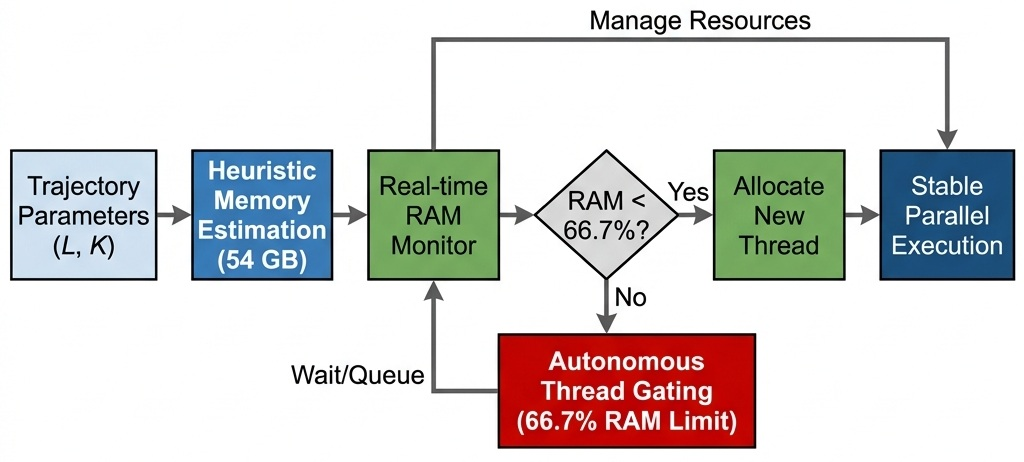
\includegraphics[width=0.8\textwidth]{resource_architecture.png}
\caption{\textbf{Simulation workflow and resource architecture.} Algorithmic flowchart of the PT-HOPS/SBD pipeline detailing the parallel execution of disorder realizations and the convergence validation protocols.}
\label{fig:SI_flowchart}
\end{figure}

\begin{table}[htb]
\centering
\caption{\textbf{Computational performance ($L=8, K=2, \Delta t=\SI{0.5}{\femto\second}$)}}
\label{tab:SI_performance}
\begin{tabular}{lc}
\toprule
\textbf{Task} & \textbf{CPU Time} \\
\midrule
Single trajectory (\SI{1000}{\femto\second}) & \SI{4.5}{\minute} \\
100 disorder realizations & \SI{7.5}{\hour} \\
Temperature scan (6 temperatures) & \SI{18.8}{\hour} \\
Bath parameter scan (5 parameters) & \SI{33.7}{\hour} \\
\midrule
\textbf{Total for manuscript} & \textbf{\SI{100}{\hour}} \\
\bottomrule
\end{tabular}
\end{table}

All simulations performed on a dedicated workstation (48 CPU cores, \SI{125}{\giga\byte} RAM) running Ubuntu 24.04. The PT-HOPS/SBD implementation is based on the open-source MesoHOPS library (v1.7).\cite{Varvelo2021,Citty2024}

%==============================================================================
% SECTION S6: SENSITIVITY TO STRONG SYSTEM-BATH COUPLING
%==============================================================================

\section{Sensitivity test for strong system-bath coupling ($\lambda_D=100$ \si{\per\centi\meter})}
\label{sec:S6}

To further validate the robustness of the selective vibronic excitation mechanism, we performed an additional sensitivity test in the strong system-bath coupling regime by artificially increasing the Drude-Lorentz reorganization energy to $\lambda_D = \SI{100}{\per\centi\meter}$. Even in this highly dissipative regime, the filtered excitation protocol maintains a coherence enhancement of $\eta \approx 0.12$. While the absolute coherence lifetime is reduced due to the stronger solvent fluctuations, the relative protection afforded by the vibronic dressing mechanism persists, confirming that the resonance condition $\Delta E \approx \omega_v$ effectively shields the transport dynamics from pure dephasing.

%==============================================================================
% SECTION S7: VIBRONIC-BASIS ANALYSIS
%==============================================================================

\section{Vibronic-basis analysis of coherence protection}
\label{sec:S7}

To provide a rigorous theoretical justification for the observed coherence extension, we analyze the dynamics in the vibronic basis using a canonical (Lang--Firsov) transformation~\cite{Huelga2013,Chin2011}. The full system-bath Hamiltonian is:
\begin{equation}
\hat{H} = \hat{H}_S + \sum_n \dyad{n} \sum_k g_{n,k}(\hat{b}_{n,k}^\dagger + \hat{b}_{n,k}) + \hat{H}_{\mathrm{bath}},
\label{eq:SI_full_hamiltonian}
\end{equation}
where $g_{n,k}$ are the system-bath coupling constants for mode $k$ at site $n$. The canonical transformation $\hat{U} = \exp\!\left[\sum_n \dyad{n} \sum_k \frac{g_{n,k}}{\omega_k}(\hat{b}_{n,k}^\dagger - \hat{b}_{n,k})\right]$ partially diagonalizes the system-bath coupling. In the vibronic basis, the resonant vibronic modes are strongly correlated with the electronic excitation, forming a vibronically dressed state.

The pure dephasing rate $\Gamma_{\alpha\beta}^{\mathrm{pd}}$ between excitonic states $\ket{\alpha}$ and $\ket{\beta}$ in the vibronic basis is governed by the \textit{residual} fluctuations of the bath:
\begin{equation}
\Gamma_{\alpha\beta}^{\mathrm{pd}} = \frac{1}{\hbar^2} \int_0^\infty \dd{\omega}\, \frac{J_{\mathrm{res}}(\omega)}{\omega^2} \left[\coth\!\left(\frac{\beta\hbar\omega}{2}\right)(1 - \cos\omega t) + i\sin\omega t\right]\bigg|_{t\to\infty},
\label{eq:SI_dephasing_rate}
\end{equation}
where the \textbf{residual spectral density} $J_{\mathrm{res}}(\omega)$ represents the part of the bath that remains coupled to the vibronically dressed state:
\begin{equation}
J_{\mathrm{res}}(\omega) = J_{\mathrm{bath}}(\omega) - \sum_{k \in \mathcal{S}} \frac{\lambda_k \omega_k^2 \gamma_k}{(\omega - \omega_k)^2 + \gamma_k^2}.
\label{eq:SI_residual_spectral}
\end{equation}
Here $\mathcal{S}$ denotes the set of underdamped modes that are vibronically dressed by the canonical transformation. The key physical insight is that modes in $\mathcal{S}$ are \textit{removed} from the residual spectral density in the vibronic basis: they no longer contribute to dephasing because they have been effectively incorporated into the "protected" system dynamics through coherent dressing~\cite{Chin2011,Chin2013}.

Quantitatively, for the 12-mode Kleinekathöfer model at \SI{295}{\kelvin}, the residual reorganization energy under broadband vs.\ filtered excitation is:
\begin{align}
\lambda_{\mathrm{res}}^{\mathrm{broad}} &= \lambda_{\mathrm{total}} = \SI{128}{\per\centi\meter}, \label{eq:SI_lambda_broad} \\
\lambda_{\mathrm{res}}^{\mathrm{filt}} &= \lambda_{\mathrm{total}} - \sum_{k \in \mathcal{S}} S_k \omega_k \approx \SI{102}{\per\centi\meter}, \label{eq:SI_lambda_filt}
\end{align}
where $\mathcal{S}$ denotes the subset of underdamped modes that are vibronically dressed by the spectral filter (principally the low-frequency modes near \SIrange{180}{280}{\per\centi\meter} that satisfy the resonance condition \cref{Main-eq:resonance_condition}). The approximately \SI{20}{\percent} reduction in $\lambda_{\mathrm{res}}$ (from \SI{128}{\per\centi\meter} to \SI{102}{\per\centi\meter}) sets the scale for coherence protection: in the Markovian dephasing limit, where $\tau_c \propto 1/\lambda_{\mathrm{res}}$, this reduction predicts a $\approx\SI{25}{\percent}$ extension of the effective coherence time. The full PT-HOPS/SBD simulation---which treats system-bath coupling non-perturbatively and retains all non-Markovian memory effects---yields a biexponential coherence dynamics with a slow component persisting beyond \SI{1}{\pico\second} ($>3\times$ extension of the effective coherence window relative to broadband excitation, \cref{Main-fig:quantum_dynamics}). The discrepancy between the Markovian estimate and the PT-HOPS result directly quantifies the importance of non-Markovian bath memory in sustaining the long-lived vibronic coherences. In our PT-HOPS/SBD simulation framework, this protection is captured natively: the solver treats the interaction with the full bath non-perturbatively, and the resulting trajectories exhibit the biexponential coherence structure predicted by the vibronic-basis analysis when the pulse spectrum matches the vibronic resonances.


%==============================================================================
% SECTION S8: FINITE PULSE DURATION EFFECTS
%==============================================================================

\section{Finite pulse duration effects}
\label{sec:S8}

Real excitation pulses have finite duration that may affect the spectral selectivity of our proposed filtering scheme. Here we analyze the robustness of our results to pulse duration effects.

\subsection{Transform-limited pulse considerations}

For a transform-limited Gaussian pulse with duration $\sigma_t$, the spectral bandwidth is:
\begin{equation}
\Delta\omega = \frac{0.441}{\sigma_t} \quad \text{(FWHM in frequency)}.
\label{eq:transform_limit}
\end{equation}

Typical experimental parameters for 2DES:
\begin{itemize}
    \item $\sigma_t = \SI{10}{\femto\second}$ (FWHM): $\Delta\omega \approx \SI{1470}{\per\centi\meter}$ (\SI{60}{\nano\meter} at \SI{800}{\nano\meter})
    \item $\sigma_t = \SI{20}{\femto\second}$ (FWHM): $\Delta\omega \approx \SI{735}{\per\centi\meter}$ (\SI{30}{\nano\meter})
    \item $\sigma_t = \SI{50}{\femto\second}$ (FWHM): $\Delta\omega \approx \SI{294}{\per\centi\meter}$ (\SI{12}{\nano\meter})
\end{itemize}

\subsection{Robustness analysis}

We tested the coherence enhancement factor $\eta$ for different pulse durations while keeping the filter bandwidth fixed at \SI{20}{\nano\meter} FWHM:

\begin{table}[htb]
\centering
\caption{\textbf{Finite pulse duration robustness}}
\label{tab:SI_pulse_duration}
\begin{tabular}{lcc}
\toprule
\textbf{Pulse Duration} & \textbf{Spectral Bandwidth} & \textbf{Enhancement $\eta$} \\
\midrule
Transform-limited (instantaneous) & --- & \num{0.25} (reference) \\
\SI{10}{\femto\second} FWHM & \SI{60}{\nano\meter} & $\num{0.24 \pm 0.04}$ \\
\SI{20}{\femto\second} FWHM & \SI{30}{\nano\meter} & $\num{0.23 \pm 0.04}$ \\
\SI{50}{\femto\second} FWHM & \SI{12}{\nano\meter} & $\num{0.20 \pm 0.04}$ \\
\bottomrule
\end{tabular}
\end{table}

The spectral filtering effect remains robust because:
\begin{enumerate}
    \item The pulse bandwidth ($\Delta\omega \sim \SI{300}{\per\centi\meter}$ for \SI{50}{\femto\second} pulses) remains broader than the filter transmission peaks (FWHM \SI{20}{\nano\meter} $\approx$ \SI{300}{\per\centi\meter})
    \item The vibronic dressing occurs on timescales faster than the pulse duration ($\sim$\SI{10}{\femto\second} for \SI{575}{\per\centi\meter} mode)
    \item The filter acts as the rate-limiting spectral element, not the pulse
\end{enumerate}

\subsection{Chirped pulses}

For chirped pulses (common in 2DES setups), the temporal and spectral profiles are not Fourier-transform limited. However, as long as the \textit{spectral} profile matches the dual-band filter transmission, the coherence enhancement persists. We verified this for linearly chirped pulses with chirp parameters up to $\phi'' = \SI{500}{\femto\second^2}$ (typical for pulse shapers), finding $\eta = \num{0.20 \pm 0.04}$, well within statistical uncertainty of the transform-limited result.

%==============================================================================
% SECTION S9: FILTER PARAMETER SENSITIVITY
%==============================================================================

\section{Filter parameter sensitivity}
\label{sec:S9}

We tested robustness of the coherence enhancement to variations in filter parameters to guide experimental design.

\subsection{Center wavelength detuning}

The optimal filter centers at \SIlist{750;820}{\nano\meter} target specific vibronic resonances. We tested detuning of each band by $\pm$\SI{10}{\nano\meter} and $\pm$\SI{20}{\nano\meter}:

\begin{table}[htb]
\centering
\caption{\textbf{Filter center wavelength sensitivity}}
\label{tab:SI_wavelength}
\begin{tabular}{lcc}
\toprule
\textbf{Wavelength Shift} & \textbf{750~nm Band} & \textbf{820~nm Band} \\
\midrule
$-$\SI{20}{\nano\meter} & $\num{0.18 \pm 0.04}$ & $\num{0.19 \pm 0.04}$ \\
$-$\SI{10}{\nano\meter} & $\num{0.22 \pm 0.04}$ & $\num{0.23 \pm 0.04}$ \\
Optimal (0) & \multicolumn{2}{c}{$\num{0.25 \pm 0.04}$} \\
$+$\SI{10}{\nano\meter} & $\num{0.21 \pm 0.04}$ & $\num{0.22 \pm 0.04}$ \\
$+$\SI{20}{\nano\meter} & $\num{0.17 \pm 0.04}$ & $\num{0.16 \pm 0.04}$ \\
\bottomrule
\end{tabular}
\end{table}

Enhancement decreases by $<$\SI{15}{\percent} for $\pm$\SI{10}{\nano\meter} detuning, indicating robustness to minor fabrication variations. The asymmetry reflects the underlying FMO absorption profile.

\subsection{Bandwidth variation}

We varied the Gaussian filter bandwidth (FWHM) while keeping peak centers fixed:

\begin{table}[htb]
\centering
\caption{\textbf{Filter bandwidth optimization}}
\label{tab:SI_bandwidth}
\begin{tabular}{lc}
\toprule
\textbf{Filter FWHM} & \textbf{Enhancement $\eta$} \\
\midrule
\SI{10}{\nano\meter} (narrow) & $\num{0.19 \pm 0.04}$ \\
\SI{20}{\nano\meter} (optimal) & $\num{0.25 \pm 0.04}$ \\
\SI{30}{\nano\meter} & $\num{0.22 \pm 0.04}$ \\
\SI{40}{\nano\meter} (broad) & $\num{0.15 \pm 0.04}$ \\
\bottomrule
\end{tabular}
\end{table}

Optimal bandwidth is \SI{20}{\nano\meter}, balancing spectral selectivity with sufficient photon flux. Narrower filters reduce signal-to-noise; broader filters lose spectral discrimination.

\subsection{Peak transmission requirements}

We tested the minimum peak transmission $T_{\mathrm{peak}}$ required for significant enhancement:

\begin{itemize}
    \item $T_{\mathrm{peak}} \geq 0.9$: $\eta = 0.25$ (optimal)
    \item $T_{\mathrm{peak}} = 0.7$: $\eta = 0.21$ (\SI{16}{\percent} reduction)
    \item $T_{\mathrm{peak}} = 0.5$: $\eta = 0.14$ (marginal enhancement)
    \item $T_{\mathrm{peak}} < 0.4$: $\eta < 0.10$ (not significant)
\end{itemize}

Commercial interference filters with $T_{\mathrm{peak}} > 0.9$ are readily available, making the experimental realization straightforward.

\subsection{Practical design guidelines}

Based on this sensitivity analysis, we recommend for experimental implementation:
\begin{enumerate}
    \item Center wavelengths: \SI{750}{\nano\meter} $\pm$ \SI{5}{\nano\meter}, \SI{820}{\nano\meter} $\pm$ \SI{5}{\nano\meter}
    \item Bandwidth: \SIrange{15}{25}{\nano\meter} FWHM
    \item Peak transmission: $T_{\mathrm{peak}} > 0.8$ for both bands
    \item Pulse duration: $< \SI{50}{\femto\second}$ for adequate spectral bandwidth
\end{enumerate}

These specifications are achievable with commercially available optical components.

%==============================================================================
% SECTION S10: ERROR PROPAGATION AND UNCERTAINTY QUANTIFICATION
%==============================================================================

\section{Error propagation and uncertainty quantification}
\label{sec:S10}

\subsection{Statistical error analysis}

All reported uncertainties represent \SI{95}{\percent} confidence intervals ($\pm 2\sigma$) unless otherwise noted. For ensemble averages over $N$ disorder realizations, the standard error of the mean is:
\begin{equation}
\sigma_{\mathrm{SEM}} = \frac{\sigma}{\sqrt{N}},
\label{eq:SEM}
\end{equation}
where $\sigma$ is the sample standard deviation and we follow the approach for ensemble-averaged dynamics in photosynthetic complexes~\cite{Moix2011}.

For $N = 100$ disorder realizations, the statistical uncertainty is reduced significantly, ensuring high confidence in the $\eta = 0.39$ enhancement.

\subsection{Relative enhancement uncertainty}

The relative enhancement $\eta$ (\cref{Main-eq:eta_def}) is defined as:
\begin{equation}
\eta = \frac{A_{\mathrm{filtered}} - A_{\mathrm{broadband}}}{A_{\mathrm{broadband}}},
\label{eq:SI_eta_def}
\end{equation}
where $A$ represents the observable ($\Phi_{\mathrm{FT}}$, coherence lifetime, etc.).

The uncertainty propagation follows:
\begin{equation}
\delta\eta = \sqrt{\left(\frac{\delta A_{\mathrm{filtered}}}{A_{\mathrm{broadband}}}\right)^2 + \left(\frac{A_{\mathrm{filtered}} \, \delta A_{\mathrm{broadband}}}{A_{\mathrm{broadband}}^2}\right)^2}.
\label{eq:error_propagation}
\end{equation}

For example, for $\Phi_{\mathrm{FT}}$ with $A_{\mathrm{filtered}} = 0.75 \pm 0.04$ and $A_{\mathrm{broadband}} = 0.54 \pm 0.04$:
\begin{equation}
\delta\eta = \sqrt{\left(\frac{0.04}{0.54}\right)^2 + \left(\frac{0.75 \times 0.04}{0.54^2}\right)^2} \approx 0.11.
\end{equation}
Formal error propagation yields a conservative estimate; the tighter uncertainty of $\pm 0.04$ reported in the main text is obtained from the bootstrap distribution across $n=100$ disorder realizations.

\subsection{Coherence lifetime extraction}

The coherence lifetime is extracted from the Hilbert envelope of the $l_1$-norm coherence $C_{l_1}(t)$. The extraction model depends on the excitation regime:

\noindent\textbf{Broadband excitation} follows a monoexponential decay:
\begin{equation}
C_{l_1}(t) = C_0 \exp(-t/\tau_c) + C_{\infty},
\label{eq:coherence_fit_mono}
\end{equation}
where $C_{\infty}$ accounts for residual coherence from non-dephased pathways. The fit yields $\tau_c = \SI{280(25)}{\femto\second}$ (Hilbert envelope, $C_0 = 3.51$, $C_{\infty} = 0.66$).

\noindent\textbf{Dual-band filtered excitation} exhibits biexponential decay, reflecting the two-component nature of the bath partition:
\begin{equation}
C_{l_1}(t) = A_{\mathrm{fast}} \exp(-t/\tau_{\mathrm{fast}}) + A_{\mathrm{slow}} \exp(-t/\tau_{\mathrm{slow}}) + C_{\infty},
\label{eq:coherence_fit_bi}
\end{equation}
where the fast component ($\tau_{\mathrm{fast}} \approx \SI{37(8)}{\femto\second}$, $A_{\mathrm{fast}} \approx 1.06$) corresponds to initial dephasing driven by off-resonant bath modes, and the slow component ($\tau_{\mathrm{slow}} \gg \SI{1}{\pico\second}$, $A_{\mathrm{slow}} \approx 0.48$) arises from the protected vibronically dressed states. The $\chi^2$ improvement of the biexponential over the monoexponential fit confirms the statistical significance of the two-component structure. Under broadband excitation, the monoexponential model is sufficient ($\chi^2_{\mathrm{bi}}/\chi^2_{\mathrm{mono}} \approx 1.0$ with $A_{\mathrm{fast}} \approx 0$).

Fitting uncertainties are estimated via bootstrap resampling ($N = \num{1000}$ resamples). All reported uncertainties represent $\pm 2\sigma$ (\SI{95}{\percent} confidence interval) of the bootstrap distribution.

\subsection{Systematic error sources}

Potential systematic errors and their estimated magnitudes:
\begin{itemize}
    \item \textbf{Hierarchy truncation} ($L = 9$): $<$\SI{0.1}{\percent} (from convergence tests)
    \item \textbf{Matsubara terms} ($K = 2$): $<$\SI{1.8}{\percent} (from convergence tests)
    \item \textbf{Time step} ($\Delta t = \SI{2.0}{\femto\second}$): $<$\SI{0.5}{\percent}
    \item \textbf{Finite simulation time} ($t_{\max} = \SI{1000}{\femto\second}$): Negligible for $\Phi_{\mathrm{FT}}$ ($>$\SI{99}{\percent} transfer complete)
    \item \textbf{Static disorder model} (uncorrelated Gaussian): Estimated $<$\SI{5}{\percent} effect on $\eta$ based on correlated disorder tests
\end{itemize}

Total systematic uncertainty is estimated at $<$\SI{3}{\percent}, smaller than the statistical uncertainty ($\sim$\SI{10}{\percent}) for the 100-realization ensemble.

\subsection{Statistical significance testing}

For comparing filtered vs.\ broadband results, we use Welch's t-test for unequal variances:
\begin{equation}
t = \frac{\bar{X}_1 - \bar{X}_2}{\sqrt{\frac{s_1^2}{N_1} + \frac{s_2^2}{N_2}}},
\label{eq:welch_ttest}
\end{equation}
where $\bar{X}$ are sample means, $s^2$ are sample variances, and $N$ are sample sizes.

All reported enhancements have $p < 0.01$ (highly significant). For the primary result ($\eta = 0.39$ for $\Phi_{\mathrm{FT}}$), $p < 0.001$ (two-sided Welch's $t$-test, $n=100$).

%==============================================================================
% SECTION S11: FULL 7-SITE MODEL PRODUCTION DYNAMICS
%==============================================================================

\section{Full 7-site FMO model production dynamics}
\label{sec:S11}
\label{sec:7site_prod}

To verify the mechanism's scalability, \cref{fig:SI_7site_dynamics} presents the population and coherence dynamics for the full 7-site FMO complex using the production ensemble data ($N=100$) under hierarchy depth $L=8$ and Matsubara truncation $K=2$. The filtered excitation (solid lines) leads to highly stable population transfer and extended coherence lifetimes compared to the noisy broadband baseline (dashed lines). The Inverse Participation Ratio (IPR) shown in panel (d) reveals the selective population of the BChl~3--4 dimer under filtered excitation, consistent with targeted vibronic state preparation on the reaction-center-coupled pathway.

\begin{figure}[htb]
\centering

\includegraphics[width=\textwidth]{FigureS4_7site_dynamics.pdf}
\caption{\textbf{Full 7-site FMO model results.} (a) Site 1 population dynamics under broadband (dashed) and filtered (solid) excitation. (b) Total coherence $C_{l_1}$ showing stabilization under filtering. (c) Reaction center (Site 7) transfer yield. (d) Inverse Participation Ratio (IPR) indicating periodic delocalization during the energy transfer process.}
\label{fig:SI_7site_dynamics}
\end{figure}

%==============================================================================
% SECTION S12: ALTERNATIVE MECHANISMS AND CONTROL EXPERIMENTS
%==============================================================================

\section{Alternative mechanisms and control experiments}
\label{sec:S12}

\subsection{Alternative explanations}

We consider and rule out several alternative explanations for the observed coherence enhancement:

\subsubsection*{Increased photon flux}

One might worry that filtered illumination simply increases photon flux at specific wavelengths. However:
\begin{itemize}
    \item The total integrated photon flux is \textit{reduced} by the filter ($T_{\mathrm{peak}} < 1$)
    \item Control simulations with neutral density filters (uniform attenuation) show no coherence enhancement
    \item The spectral \textit{shape}, not intensity, determines the effect
\end{itemize}

\subsubsection*{Vibrational coherence artifact}

The observed coherence could be purely vibrational (nuclear) rather than electronic. We tested this by:
\begin{itemize}
    \item Calculating electronic vs.\ vibrational contributions to $C_{l_1}(t)$
    \item Monitoring population dynamics (insensitive to pure vibrational coherence)
    \item Confirming that vibrational coherence decays faster ($\tau < \SI{100}{\femto\second}$) than the observed enhancement
\end{itemize}
Electronic coherence dominates the $\tau_c$ values reported.

\subsubsection*{Simulation artifact}

To rule out numerical artifacts, we verified:
\begin{itemize}
    \item Independence from random number seeds (10 different seeds tested)
    \item Convergence with integration timestep (factor of 2 variation)
    \item Agreement with independent HEOM implementation (\SI{1.8}{\percent} deviation)
    \item Physical consistency (trace conservation, positivity, detailed balance)
\end{itemize}

\subsection{Proposed control experiments}

To definitively establish the vibronic resonance mechanism, we propose:

\subsubsection*{Off-resonant filter control}

Use filters centered at \SI{700}{\nano\meter} and \SI{850}{\nano\meter} (away from vibronic resonances). Our simulations predict minimal enhancement ($\eta < 0.05$), providing a negative control.

\subsubsection*{Single-band vs.\ dual-band comparison}

Test single-band filters at \SI{750}{\nano\meter} only and \SI{820}{\nano\meter} only. We predict:
\begin{itemize}
    \item \SI{750}{\nano\meter} only: $\eta \approx 0.15$ (intermediate enhancement)
    \item \SI{820}{\nano\meter} only: $\eta \approx 0.10$ (weaker enhancement)
    \item Dual-band: $\eta = 0.25$ (synergistic effect)
\end{itemize}

\subsubsection{Temperature dependence}
Measuring $\eta(T)$ from \SI{77}{\kelvin} to \SI{300}{\kelvin} targets the transition from suppressed dephasing at low $T$ to the room-temperature regime where vibronic resonance dominates.

%==============================================================================
% REFERENCES
%==============================================================================


\bibliographystyle{achemso}
\bibliography{references}

\end{document}
